% LARGE SCALE

\documentclass[preprint]{sigplanconf}

\usepackage{amsmath}
\usepackage{listings}
\usepackage{float}
\usepackage{graphicx}
\usepackage{adjustbox}
\usepackage{multirow}
\usepackage{color}


\newcommand{\lyxdot}{.}

\floatstyle{ruled}
\newfloat{Listing}{tbp}{loa}

\begin{document}

\special{papersize=8.5in,11in}
\setlength{\pdfpageheight}{\paperheight}
\setlength{\pdfpagewidth}{\paperwidth}

\conferenceinfo{CONF 'yy}{Month d--d, 20yy, City, ST, Country} 
\copyrightyear{20yy} 
\copyrightdata{978-1-nnnn-nnnn-n/yy/mm} 
\doi{nnnnnnn.nnnnnnn}

% Uncomment one of the following two, if you are not going for the 
% traditional copyright transfer agreement.

%\exclusivelicense                % ACM gets exclusive license to publish, 
                                  % you retain copyright

%\permissiontopublish             % ACM gets nonexclusive license to publish
                                  % (paid open-access papers, 
                                  % short abstracts)

%\titlebanner{banner above paper title}        % These are ignored unless
%\preprintfooter{short description of paper}   % 'preprint' option specified.

\title{How Do Programmers Use Optional Typing? A Case Study}

\authorinfo{Carlos Souza}
           {Federal University of Minas Gerais}
           {carlosgsouza@gmail.com}
\authorinfo{Eduardo Figueiredo}
           {Federal University of Minas Gerais}
           {figureido@dcc.ufmg.br}

\maketitle

\begin{abstract}
The typing system is one of the most important things to be taken in consideration when choosing a programming language. 
This question has become increasingly more important due to the recent popularization of dynamically typed languages such as Ruby and JavaScript. 
This paper presents a large scale case study with the goal of finding what are the most influential factors for a programmer when choosing between different typing paradigms. 
An analysis of the source code of over seven thousand projects written in Groovy, a programming language which features optional typing, shows in which situations programmers prefer typing or not their declarations. 
Results suggest that the need for maintainability, frequency of change and programmers background are important factors in this decision.
\end{abstract}

\category{D.2.3}{Software Engineering}{Cooding Tools and Techniques}

\terms
Experimentation, Language

\keywords
Type systems, static analysis, Groovy and GitHub

\section{Introduction}
When choosing a programming language for a project, a developer considers several characteristics of that language.
One of the most important of these characteristics is its typing system, which can be static or dynamic.
The typing system determines when the type of a statement is defined \cite{types_and_programming_languages}. 
Statically typed languages, such as Java and C\#, require the type of a statement to be defined by the programmer, which can then be used by the compiler to check for any typing errors. 
On the other side, in dynamically typed languages, like Ruby and JavaScript, the definition of the type of a statement only happens at run time.

Discussions about what is the best typing system for a particular situation have become increasingly more important in recent years due to rapid popularization of dynamically typed languages. 
According to the TIOBE Programming Community Index \cite{tiobe}, a well-known ranking that measures the popularity of programming languages, 27\% of the programming languages used in the industry are dynamically typed. 
A decade ago, this number was only 17\%. 
Among the 10 languages on top of the ranking, four are dynamically typed: JavaScript, Perl, Python and PHP. 
None of these languages were among the top 10 rank until 1998.

Several factors may be considered when choosing between a dynamically or statically typed language. 
Since dynamically typed languages are simpler, they allow programmers to code faster \cite{types_and_programming_languages} and adapt to frequently changing requirements more easily \cite{gradual_typing}.
Also, by removing the repetitive work of defining types, these languages allow programmers to focus on the problem to be solved rather than on the rules of the language \cite{dynamically_typed_languages}.

Statically typed languages also have their advantages. 
For instance, they allow compilers to find type errors statically \cite{should_your_specification_language_be_typed}. 
Typed declarations increase the maintainability of systems because they implicitly document the code, telling programmers about the nature of statements \cite{type_systems,mayer2012static}. 
Systems built with these languages tend to be more efficient since they do not need to perform type checking during their execution \cite{bruce2002foundations,jit}. 
Finally, modern development environments, such as Eclipse and IDEA, are able to assist programmers with functionalities such as code completion based on the information
provided by statically typed declarations \cite{bruch2009learning}.

Some languages try to combine characteristics from both static and dynamic type systems.
Groovy\cite{groovy} is one of these languages.
Although Groovy is mostly a dynamically typed language, it gives programmers the option to annotate their declarations with types.
It is also possible to turn static type checking so the compiler can find type errors before execution.
This allows developers to choose the most appropriate paradigm for each situation.

Understanding what are the most relevant factors on the choice for a typing system is an important matter.
Programmers can make an informed decision by knowing which languages provide the right benefits for their particular context.
Programming language developers can consider this information in their design so they can develop the most appropriate features for their target audience.
Finally, tools can be developed or improved to overcome any weaknesses of a given language. 

This paper presents a large scale case study aiming to understand which factors actually influence the decision of a developer for typing their declarations or not. 
This question was studied based on the analysis of a massive dataset with more than seven thousand Groovy projects.
Through a static analysis of these projects, it was possible to understand when developers choose each used types and then extract what are the factors that influence this decision.

Results show that programmers consider types as a means to document their code.
This is even more evident on the definition of the interface of modules.
Conversely, when readability or stability are not a concern, programmers tend to type their declarations less often.
In addition to that, programmers seem to prefer the flexibility of untyped declarations in frequently changed code.
Finally, the experience of a programmer with other languages has a relevant effect on his or her choice for typing a declaration or not.

The remainder of this paper is organized as follows. 
Section \ref{groovy} introduces the main concepts of the Groovy programming language and Section \ref{settings} presents the study settings.
Section \ref{results} describes the results of the study, which are then discussed in Section \ref{discussion}.
Some threats to the validity of this study are presented in Section \ref{threats}.
Finally, Section \ref{conclusion} concludes this study and suggests future works.












%
%  THE GROOVY LANGUAGE
%

\section{The Groovy Language\label{groovy}}
Groovy is a dynamically typed programming language which allows programmers to optionally type their declarations.
It was designed to run on the Java Virtual Machine and its adoption has grown remarkably over the last years, specially among Java developers who seek more dynamism without having to learn a completely new language.
It builds upon the strengths of Java, but has additional features inspired by dynamic languages such as Python and Ruby.

Despite having been launched less than ten years ago, Groovy is already a very popular language.
According to the TIOBE Programming Index, Groovy is the 22\textsuperscript{nd} most popular language in the software industry\cite{tiobe}, ahead of languages like Prolog, Haskell and Scala. 

The syntax of the Groovy language is similar to Java's and most of Java code is also valid in Groovy.
Like Java, Groovy code is compiled to bytecode, allowing it to seamlessly integrate with existing Java classes and libraries. 
These factors have attracted a large number of Java programmers who want to use Groovy's dynamic functionality without having to learn a completely different language or change the execution platform of their systems. 

Groovy was designed to be more expressive and concise than Java.
Two implementations of a simple algorithm are shown below.
Given a list of numbers, return a list containing only the even numbers of that list.
Listing \ref{javaClass} shows the Java implementation while Listing \ref{groovyClass} shows the Groovy counterpart. 

Because of its high level of expressiveness, Groovy is able to reduce much of the boilerplate required in Java.
Listing \ref{groovyClass} shows that Groovy offers a native syntax for lists(lines 3, 6 and 14) and operator overloading (line 6). 
Semicolons are optional, except when there are multiple statements in the same line. 
When the keyword $return$ is omitted (line 10), the last expression evaluated with a method is returned. 
Also, parenthesis in method calls can often be omitted (line 16).
In addition to that, Groovy implicitly imports frequently used classes, like those of the $java.util$ package, and methods, like $System.out.println$ (line 16).

\begin{Listing}[ht]
\begin{lstlisting}[language=Java,tabsize=2,breaklines=true,numbers=left]
import java.util.ArrayList;
import java.util.List;

public class JavaFilter {
	List<Integer> evenNumbers(List<Integer> list) {
		List<Integer> result = new ArrayList<Integer>();
		for(int item : list) {
			if(item % 2 == 0) {
				result.add(item);
			}
		}

		return result;
	}

	public static void main(String[] args) {
		List<Integer> list = new ArrayList<Integer>();
		list.add(1);
		list.add(2);
		list.add(3);
		list.add(4);

		List<Integer> result = new JavaFilter().evenNumbers(list);
		System.out.println(result);
	}
}
\end{lstlisting}
\caption{A simple algorithm written in Java}
\label{javaClass}
\end{Listing}

\begin{Listing}[ht]
\begin{lstlisting}[language=Java,tabsize=2,breaklines=true,numbers=left]
class GroovyFilter {
	List<Integer> evenNumbers(List<Integer> list) {
		List<Integer> result = []
		for(int item : list) {
			if(item % 2 == 0) {
				result << item
			}
		}

		result
	}

	public static void main(String[] args) {
		List<Integer> list = [1, 2, 3, 4]
		List<Integer> result = new GroovyFilter().evenNumbers(list)
		println result
	}
}
\end{lstlisting}
\caption{A simple algorithm written in Groovy}
\label{groovyClass}
\end{Listing}

The design of Groovy was influenced by dynamic features of programming languages such as Ruby and Python.
Listing \ref{dynamicInfuence} shows how these features can be used to rewrite the same algorithm presented in Listing \ref{javaClass} in a single line of code. 
First, notice that the code shown in Listing \ref{dynamicInfuence}  is a script, rather than a class file.
It makes use of a closure to allow a programmer to define a filter logic.
This closure is passed down to the $findAll$ method, which  apply this closure to every element of the list to in order to decide if that element should be returned or not.
Closures are one of the most important features of Groovy compared to Java.
They allow a functional programming style of code, which is both expressive and powerful.

\begin{Listing}[ht]
\begin{lstlisting}[language=Java,tabsize=2,breaklines=true,numbers=left]
println([1, 2, 3, 4].findAll {it % 2 == 0})
\end{lstlisting}
\caption{A class written in Groovy}
\label{dynamicInfuence}
\end{Listing}

Metaprogramming is another dynamic feature present in Groovy. 
Listing \ref{metaprogramming} shows how to add a method to an existing class dynamically.
By adding the method $evenNumbers()$ to the $List$ class, it is possible to achieve higher expressiveness.
This is specially useful when implementing Domain Specific Languages \cite{fowler10}.

\begin{Listing}[ht]
\begin{lstlisting}[language=Java,tabsize=2,breaklines=true,numbers=left]
List.metaClass.evenNumbers = {
	delegate.findAll {it % 2 == 0}
}
println([1, 2, 3, 4].evenNumbers())

\end{lstlisting}
\caption{An example of metaprogramming in Groovy}
\label{metaprogramming}
\end{Listing}

When Groovy 1.0 was first launched, in 2007, it was a purely dynamically typed language.
However, it allowed programmers to optionally type their statements.
Examples of typed and untyped declarations combined flexibly in the same file are shown on Listing \ref{dynamicTyping}.


\begin{Listing}[ht]
\begin{lstlisting}[language=Java,tabsize=2,breaklines=true,numbers=left]
class DynamicTyping {
	private String typedField
	private untypedField

	DynamicTyping(typedParam) {}

	def untypedMethod(untypedParam, int typedParam) {
		def untypedVariable = 1.0
		return untypedVariable
	}

	int typedMethod()  {
		String typedVariable = ""
		return typedVariable
	}
}
\end{lstlisting}
\caption{Groovy is a dynamic language}
\label{dynamicTyping}
\end{Listing}

This kind of typing should not be confused with static typing since Groovy compiler does not use these type annotations to look for errors.
For example, the snippet of code shown in Listing \ref{typeError} compiles without any errors.
During runtime, the $string$ variable references an instance of the $Integer$ class.
However, an exception is thrown when we try to invoke the method $toUpperCase$ since the $Integer$ class does not have this method.

\begin{Listing}[ht]
\begin{lstlisting}[language=Java,tabsize=2,breaklines=true,numbers=left]
String string = new Integer(1)
string.toUpperCase()
\end{lstlisting}
\caption{A class written in Groovy}
\label{typeError}
\end{Listing}

Since version 2.0, Groovy allows programmers to explicitly activate static typing with the usage of the $@TypeChecked$ annotation.
This makes Groovy a gradually typed language \cite{gray05,gray08,gray11,siek07,takikawa12}.
In this mode, the Groovy compiler looks for type errors and fail if it finds any.

Listing \ref{staticTyping} shows an example of static typing in Groovy.
Trying to compile the class $TypeCheckedGroovyClass$ produces an error since the method $sum$ is supposed to receive two parameters of the type $int$, but it is actually called with two parameters of the type $String$.

\begin{Listing}[ht]
\begin{lstlisting}[language=Java,tabsize=2,breaklines=true,numbers=left]
@TypeChecked
class TypeCheckedGroovyClass {
	
	static int sum(int a, int b) {
		a + b
	}

	public static void main(String[] args) {
		println sum("1", "2")
	}
}
\end{lstlisting}
\caption{A class written in Groovy}
\label{staticTyping}
\end{Listing}

The $@TypeChecked$ annotation is reasonably recent and most Groovy programmers still do not use it. 
Typing annotations on the other side are very popular.
Although they do not provide static type checking, they are capable of documenting the code and aiding in the integration with development tools.
In the remainder of this text, we refer to declarations with type annotations as "typed", while the word "untyped" is used for declarations with no type annotations.







%
% STUDY SETTINGS
%

\section{Setudy Settings\label{settings}}
In this paper, we conduct a case study with the goal of understanding what are the factors that have an actual influence over the decision of a developer to type their declarations or not. 
We analyze the source code of more than 7 thousand Groovy projects and find where types are used.
In the remainder of this section, we present the study settings starting by the research questions, listed in Subsection \ref{questions}. 
The Data Collection procedure is described in Subsection \ref{dataCollection} while the dataset itself is detailed in Subsection \ref{dataset}. 
Finally, we discuss the static code analyzer and the analysis procedure in Subsection \ref{analyzer}.

\subsection{Research Questoins\label{questions}}
Static and dynamic type system have known advantages and disadvantages.
We propose some research questions below in order to find which ones are actually considered by programmers in their code.

\begin{itemize}
	\item \textbf{Question Q1: Do programmers use types to implicitly document their code?} By typing their statements, developers are telling their colleagues about the nature of those statements. This increases the readability and, hence, the maintainability of their code. If we are able to observe a higher usage of types in statements that usually require more documentation, then we can assume that these developers indeed consider types as a means to document their code.
	\item \textbf{Question Q2: Are untyped declarations preferred when readability or stability are not a concern?} Besides readability, typing also contributes to stability. It reduces the risk of unexpected effects of modifications increasing the maintainability of the software system \cite{Iso2004}. Our hypothesis is that, where these aren't important factors, typing becomes less necessary and developers prefer the flexibility and objectivity offered by dynamic typing. 
	\item \textbf{Question Q3: Does the previous experience of programmers with other languages influence their choice for typing their code?} We believe that programmers familiar with a statically typed language keep using types since they get used to it. 
\end{itemize}

\subsection{Data Collection Procedure\label{dataCollection}}
The projects used in this study were obtained from GitHub, a popular source control service based on Git.
For each project, it was necessary to retrieve its source code, its metadata, and the metadata of all developers involved in that project.
GitHub does not offer a listing of all hosted projects, but it offers two search mechanisms, a REST API and a web based search page.
Unfortunately GitHub API is too limited for our requirements.
It imposes a limit of one thousand results and does not allow filtering projects by their programming language.

In order to retrieve a expressive dataset, it was necessary to write a bot to simulate human interactions with the GitHub webpage and search for projects. 
Some special care was necessary to make this work. 
For instance, because the number of results is limited to 1 thousand projects, we had to segment the queries.
Multiple requests were made, and each one asking for the name of all projects created on a given month.
Results were then combined into a single list.
Another problem faced was that GitHub denies excessive requests from the same client.
By adding a 10 seconds delay between requests, it was possible to overcome this limitation.

With the name of all projects in hands, it was then possible to use the GitHub REST API to query the metadata of all projects.
Since the metadata of a project also contains the identification of the developers of that project, it was possible to obtain the metadata of those developers using the same API.

%DATASET
\subsection{Dataset\label{dataset}}

% count scripts, main classes and test classes

Our dataset consists of 7268 Groovy projects obtained from GitHub. 
These projects include a total of 9.8 million lines of code and approximately 169 thousand Groovy files. 
There are about 412 thousand declarations considering variables, methods and fields. 
Figures \ref{fig:size_distribution} shows the cumulative distribution of the size of all these projects.
Notice that a logarithm scale is used.
Although most of the projects are relatively small, there are projects with up to 150 KLoC. 

% The age of a project, defined as the time between the first and last commits, varies form 1 day to 5 years. 
% Figure \ref{fig:age_distribution} shows the cumulative distribution of the age of the projects in the dataset. 


\begin{figure}[ht]
\centering 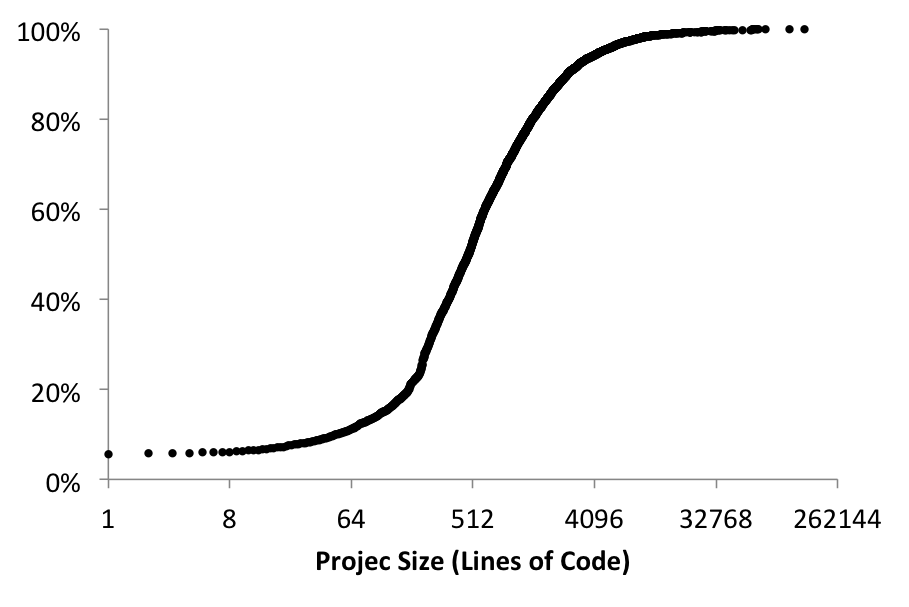
\includegraphics[width=0.45\textwidth]{images/size_distribution}
\caption{Cumulative Distribution of the Size of the Projects}
\label{fig:size_distribution} 
\end{figure}

% \begin{figure}[ht]
% \centering 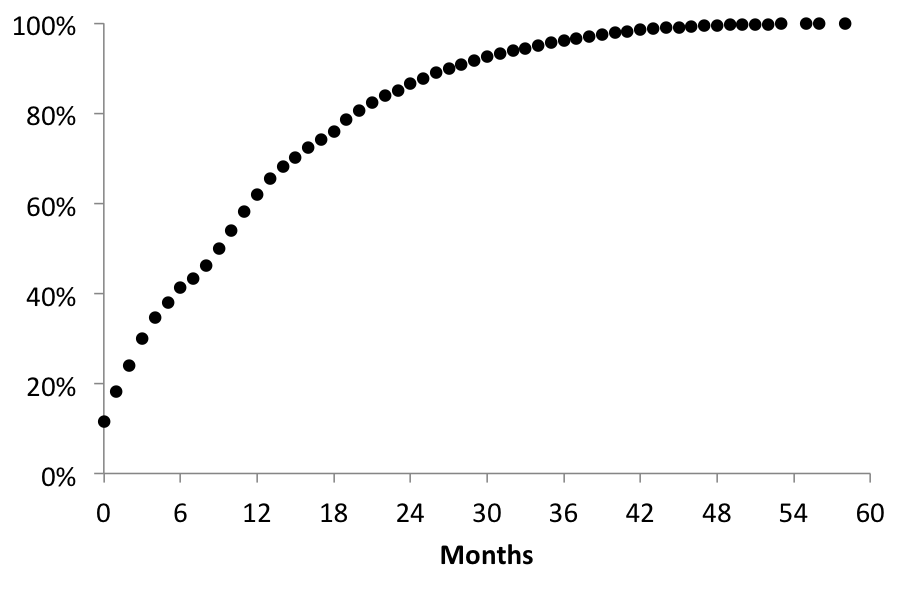
\includegraphics[width=0.45\textwidth]{images/age_distribution}
% \caption{Cumulative Distribution of the Age of the Projects}
% \label{fig:age_distribution} 
% \end{figure}

The projects in our dataset were developed by 4481 different people. 
Table \ref{tab:number_of_developers} shows that most projects were developed by a single person.
A total of 96\% of the projects were developed by small groups of 3 people or less.
However, there were projects with up to 58 people.

These developes of the 7268 projects have different backgrounds.
Figure \ref{fig:other_languages} shows what are the languages used by these developers in other GitHub projects. 
Java is the most popular among them.
More than 50\% of the developers of projects in our dataset also have Java projects hosted on GitHub.

Figure \ref{fig:typeSystem_background} shows what is the type system of the languages the developers in our dataset have experience with.
Most of them have experience with both statically and dynamically typed languages.
There are two small groups however that have experience with only one type system outside Groovy.
 
\begin{table}[ht]
\caption{Distribution of the Number of Developers in a Project}
\centering{}%
\begin{tabular}{|c|c|c|}
\hline 
Number of Developers & Fraction of Projects\tabularnewline
\hline 
\hline 
1 & 84\%\tabularnewline
\hline 
2 & 9\%\tabularnewline
\hline 
3 & 3\%\tabularnewline
\hline 
4 or more & 4\%\tabularnewline
\hline 
\end{tabular}
\label{tab:number_of_developers}
\end{table}

\begin{figure}[ht]
\centering 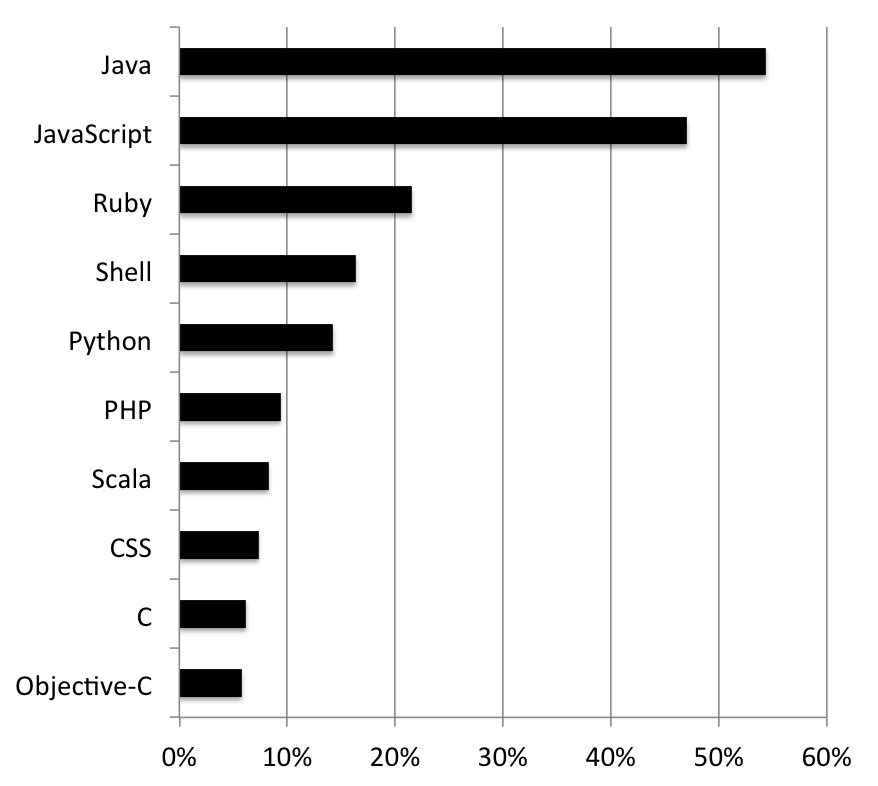
\includegraphics[width=0.45\textwidth]{images/other_languages}
\caption{Usage of other languages by Groovy developers on GitHub}
\label{fig:other_languages} 
\end{figure}

\begin{figure}[ht]
\centering 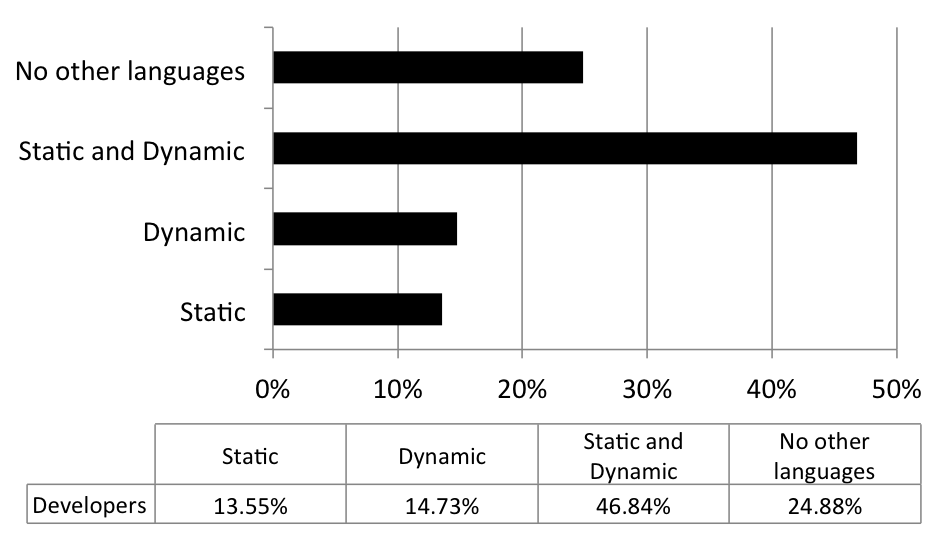
\includegraphics[width=0.45\textwidth]{images/typeSystem_background}
\caption{Type System of other languages used by programmers}
\label{fig:typeSystem_background} 
\end{figure}



%ANALYSIS
\subsection{Analysis\label{analyzer}}
In order to understand where programmers use types, a static code analyzer was built. 
This analyzer is based on the Groovy metaprogramming library, which is capable of compiling Groovy files and generate an abstract syntax tree (AST) for them.
The following types of declarations can be extracted

\begin{itemize}
	\item Method Returns
	\item Method Parameters
	\item Constructor Parameters
	\item Fields
	\item Local Variables
\end{itemize}

In addition to the declarations extracted, we rely on the static code analyzer to answer the following questions:

\begin{itemize}
	\item What is the typing system of the statement?
	\item Is the statement part of a script or a class?
	\item Is the statement part of a test class?
	\item What is the visibility of the method or field?
\end{itemize}


A relevant decision we made was no to compile projects.
We made this decision because compiling the projects would require all dependencies to be resolved, which would be unfeasible.
This would be even harder when we consider the dimension of our dataset.
Instead, we generated the AST for each file using the $CONVERSION$ phase of the Groovy compiler.
At this phase, the compiler hasn not tried to resolve any dependencies yet, but it is capable of generating an AST with sufficient information to determine if a statement had its type defined by the programmer or not.
This makes it possible to analyze each Groovy file separately without having to compile the whole project.

The downside of the approach described above is that we can not analyze Groovy code in conjunction with its dependencies. 
For example, it is impossible to answer if programmers tend to type code that interacts with other typed modules since we haven not resolved any dependencies to these modules.
However, our choice was fundamental in order to execute a study with such an expressive dataset.
Nevertheless, as shown in the next section, we were still able to obtain detailed and relevant results using this strategy.











%
% RESULTS
%
\section{Results\label{results}}
This section presents the results of our analysis showing where Groovy programmers use types and where they do not.
As an overall result, Groovy programmers use types in 60\% of their declarations.
Subsection \ref{res-type} shows the type usage in different sorts of declarations and Subsection \ref{res-visibility} details these results by visibility. Subsection \ref{res-size} shows how the project size affects the usage of types.
Subsection \ref{res-tests-scripts} present type usage in test classes and scripts. Finally, results are shown according to programmers background in Subsection \ref{res-background}.

% TYPE
\subsection{Declaration Type\label{res-type}}
Figure \ref{fig:tipo_declaracao} shows the amount of typed and untyped declarations for each sort of declaration. 
Untyped declarations are far more frequent in local variables that in other elements.
Fields, method returns and parameters on the other side are mostly typed. In particular, constructor parameters are typed in more than $90\%$ of the declarations.

\begin{figure}[h]
\centering 
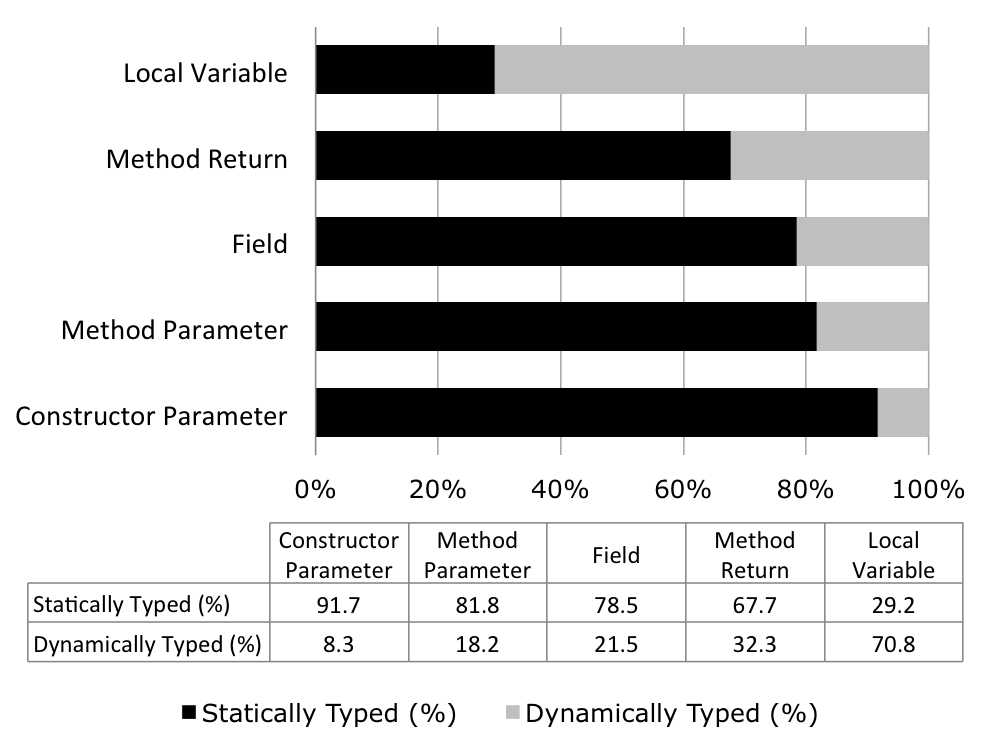
\includegraphics[width=0.45\textwidth]{images/type} 
\caption{Type Systems by Declaration Type.}
\label{fig:tipo_declaracao} 
\end{figure}

% VISIBILITY
\subsection{Visibility\label{res-visibility}}
In this section, we break down the results shown above by visibility. 
The goal is to investigate the impact of visibility on the programmers choice of typing or not.
Figure \ref{fig:method_return_visibility} shows results for method returns.
There is little difference in the usage of types on the declarations of the return in private and public methods, with $64.4\%$ and $67.3\%$ declarations typed respectively.
On the other side, the return of protected methods typed in $91.8\%$ of the cases.

\begin{figure}[h]
\centering 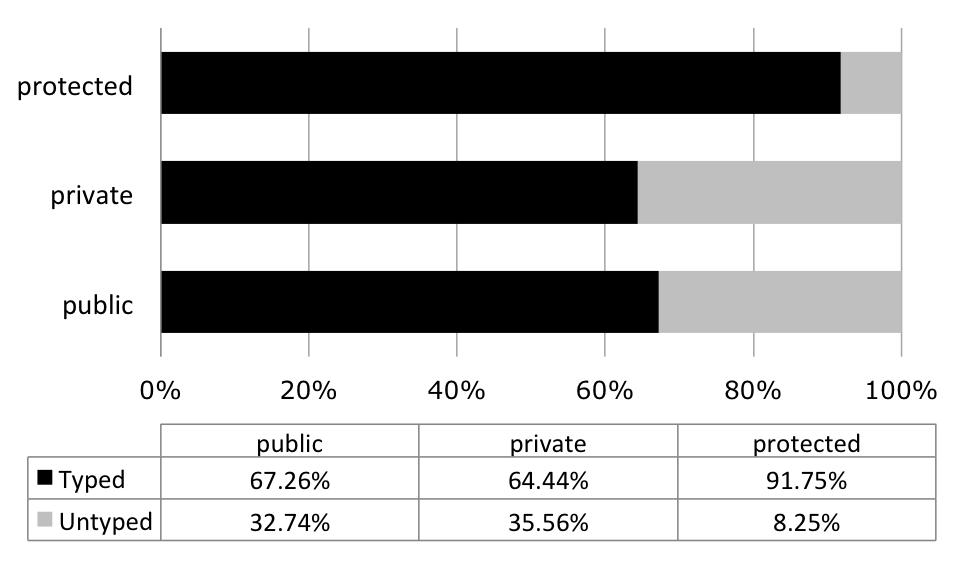
\includegraphics[width=0.45\textwidth]{images/method_return_visibility} 
\caption{Method return declarations by visibility}
\label{fig:method_return_visibility} 
\end{figure}

Figure \ref{fig:method_parameter_visibility} shows the results of the analysis of method parameter declarations. 
Compared to the results for method returns shown in Figure \ref{fig:method_return_visibility}, declarations of public method parameters are typed more often.
While public method returns have types in $67.3\%$ of the times, public method parameters have  $82.4\%$ of their declarations typed. 
Parameters of constructors, shown in Figure \ref{fig:constructor_parameter_visibility}, present a similar behavior to what we observed in parameters of methods.

\begin{figure}[h]
\centering 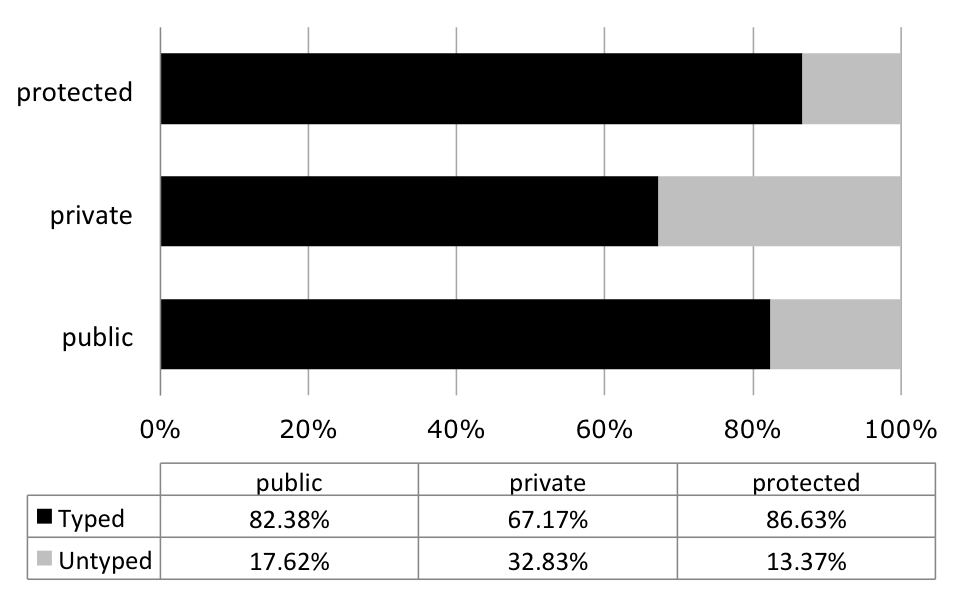
\includegraphics[width=0.45\textwidth]{images/method_parameter_visibility} 
\caption{Method parameter declarations by visibility}
\label{fig:method_parameter_visibility} 
\end{figure}


\begin{figure}[h]
\centering 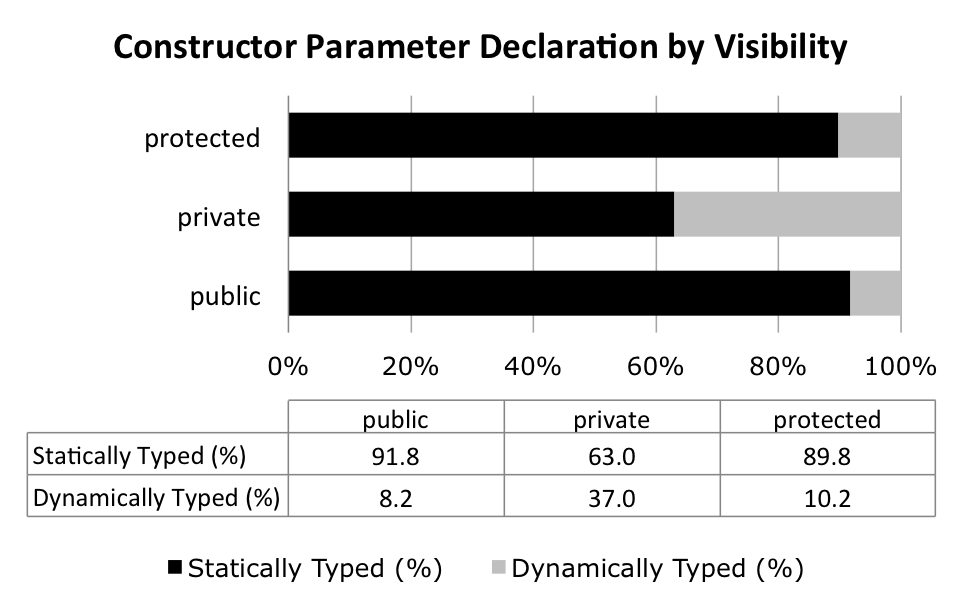
\includegraphics[width=0.45\textwidth]{images/constructor_parameter_visibility} 
\caption{Constructor parameter declaration by visibility}
\label{fig:constructor_parameter_visibility} 
\end{figure}


Figure \ref{fig:field_visibility} shows the results for field declarations. 
Differently from previous analyzed declarations, protected fields are significantly less typed than public fields. 
While the first are typed in $80.5\%$ of the cases, $88.8\%$ of the latter are typed.
Another difference is that private fields are slightly more typed than other private declarations.
This frequency is $72.4\%$ for private fields, but for method returns, method parameters, and constructor parameters it does not exceed $67\%$.


\begin{figure}[h]
\centering 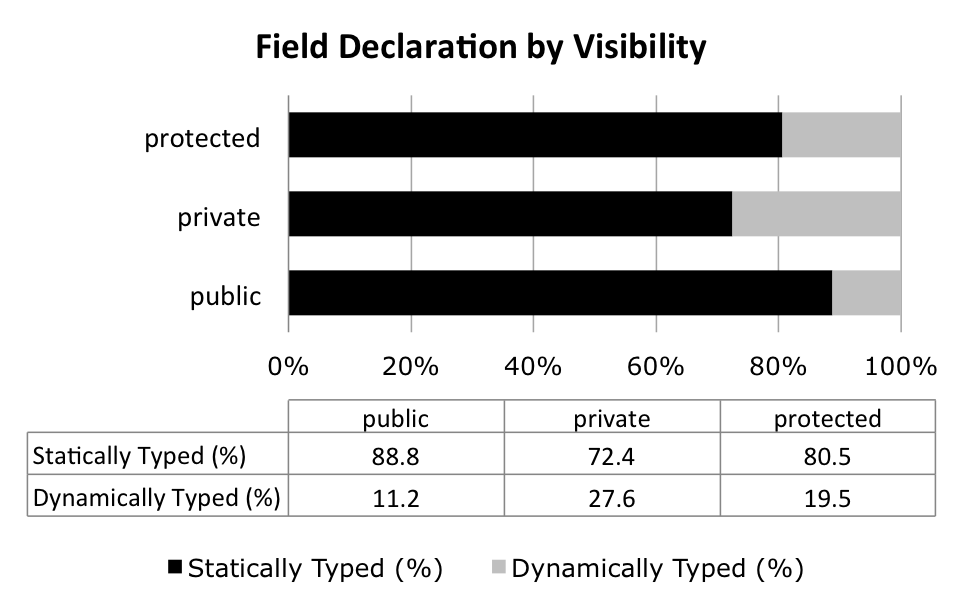
\includegraphics[width=0.45\textwidth]{images/field_visibility} 
\caption{Field declaration by visibility}
\label{fig:field_visibility} 
\end{figure}

In summary, for all types of declarations, private declarations are less typed than the public and protected counterparts.
Protected declarations, on the other side, are usually the most typed. The only exception to this are fields, where the usage of types in public declarations surpasses those of protected declarations by $8\%$.

% TESTS
\subsection{Scripts and Test Classes\label{res-tests}}
In this section, we analyze how types are used in test classes and scripts.
Figure \ref{fig:test_classes} shows that declarations in test classes are typed in 55.9\% of the cases.
Meanwhile, main classes have 67.8\% of their declarations typed.
The difference between these two types of classes is about $14\%$.

\begin{figure}[ht]
\centering 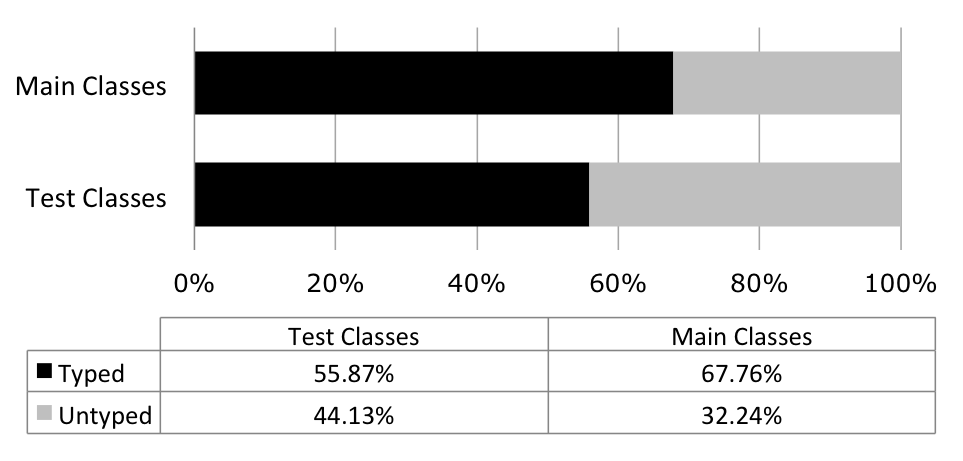
\includegraphics[width=0.45\textwidth]{images/test_classes} 
\caption{Declarations in test classes and main classes}
\label{fig:test_classes} 
\end{figure}

As shown in Figure \ref{fig:scripts}, scripts present a different behavior.
Classes are typed in 58.6\% of the cases. This number is 63.6\%. for scripts.
With a difference inferior to 5\%, we can say that classes and scripts present equivalent behaviors.

\begin{figure}[ht]
\centering 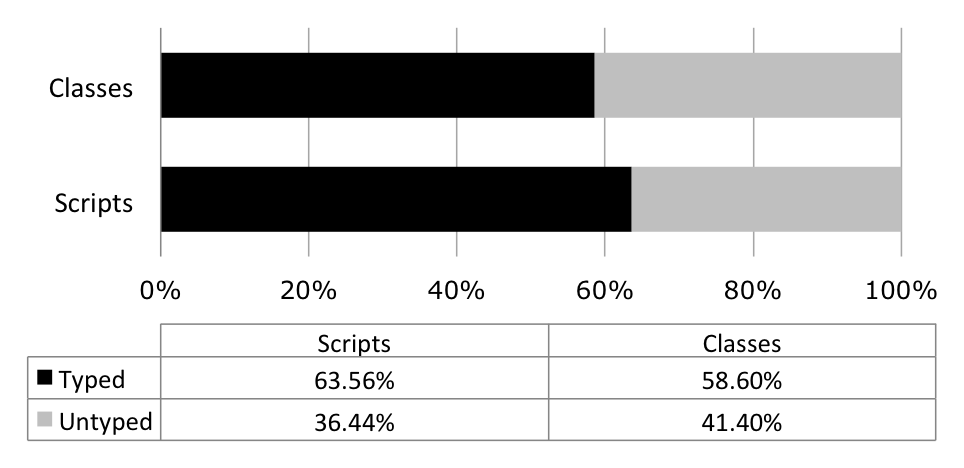
\includegraphics[width=0.45\textwidth]{images/scripts} 
\caption{Declarations in scripts and classes}
\label{fig:scripts} 
\end{figure}


% PROGRAMMERS BACKGROUND
\subsection{Programmers Background\label{res-background}}

Figure \ref{fig:untyped_background} shows how programmers use types in their statements according to the type system of the languages they have used on GitHub.
Developers are distributed in three groups, those with only statically typed languages, those with only dynamically dynamic languages and those with both. 

There is a clear distinction in the behavior of those whose all projects are written in statically typed languages.
These programmers use types in about 28\% of their statements compared to 40\% of the other programmers.
Notice that the behavior of those programmers with only dynamic languages on their portfolio is no different from those with statically and dynamically typed languages.

\begin{figure}[ht]
\centering 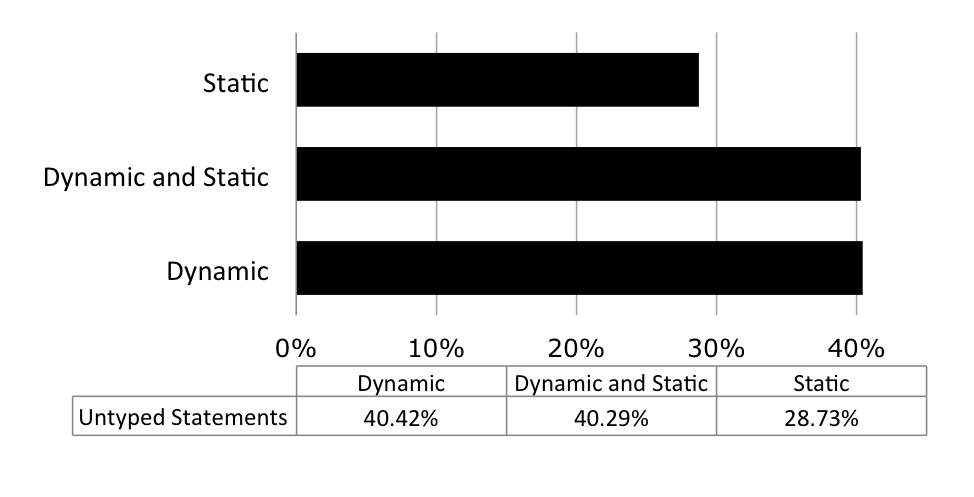
\includegraphics[width=0.45\textwidth]{images/untyped_background} 
\caption{Programmers Background and Usage of Untyped Declarations}
\label{fig:untyped_background} 
\end{figure}

% PROJECT SIZE
\subsection{Project Size\label{res-size}}
In this section we present the results for the use of types in declarations as projects grown in size.
The project size is a simple metric to measure the complexity of a project.
Usually, the larger the project, the greater the number of modules and the need for maintenance \cite{Fenton1998}. 

Figure \ref{fig:size_pubMethodReturn} shows the how the frequency of untyped declarations in public statements varies with the project size.
In this graph, each bar shows the average usage of untyped declarations of projects grouped by their size.
The boundaries of each group are defined under each bar.
For example, a project with $1500$ lines of code is in the fifth group, since $1500$ lies within the interval $]1024, 2048]$.
Notice that we are using a logarithm scale for the project size in these graphs.
Types are less used in public declarations as project size increases.
While projects with less than $1024$ lines of code have almost $40\%$ of their declarations untyped, this number is  less than $20\%$ in projects with over $65536$ lines of code. 

Figure \ref{fig:size_priMethodReturn} shows that, different from public declarations, private declarations have no apparent correlation with the project size. 
The same can be said for protected declarations, which are shown in Figure \ref{fig:size_proMethodReturn}.

\begin{figure*}[ht]
\centering 
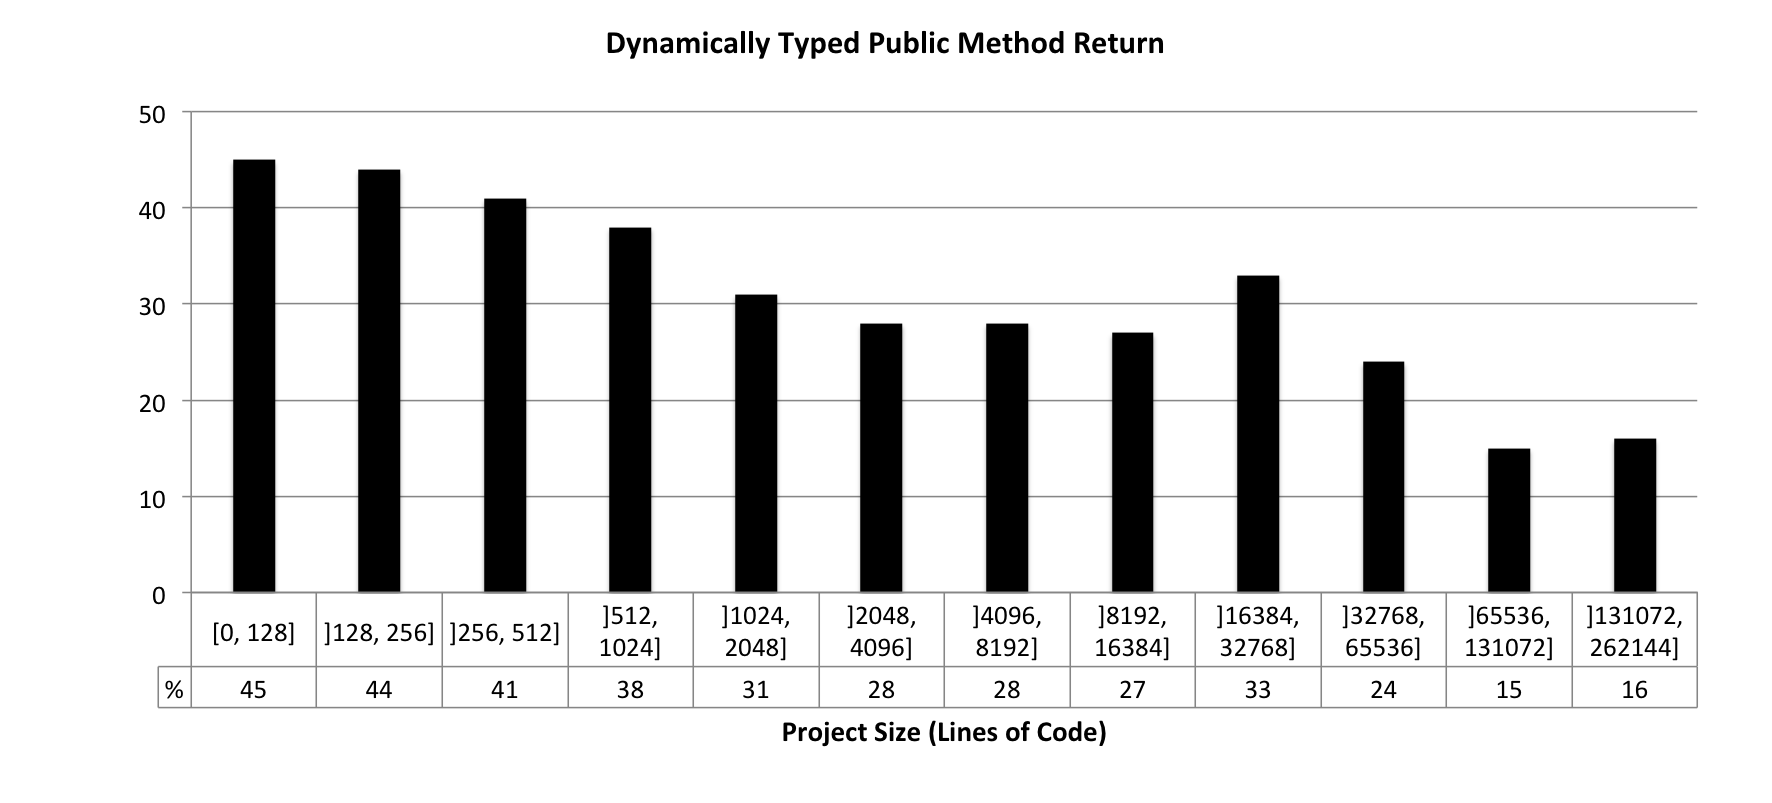
\includegraphics[width=1\textwidth]{images/size_pubMethodReturn} 
\caption{Untyped public declarations}
\label{fig:size_pubMethodReturn} 
\end{figure*}

\begin{figure*}[ht]
\centering 
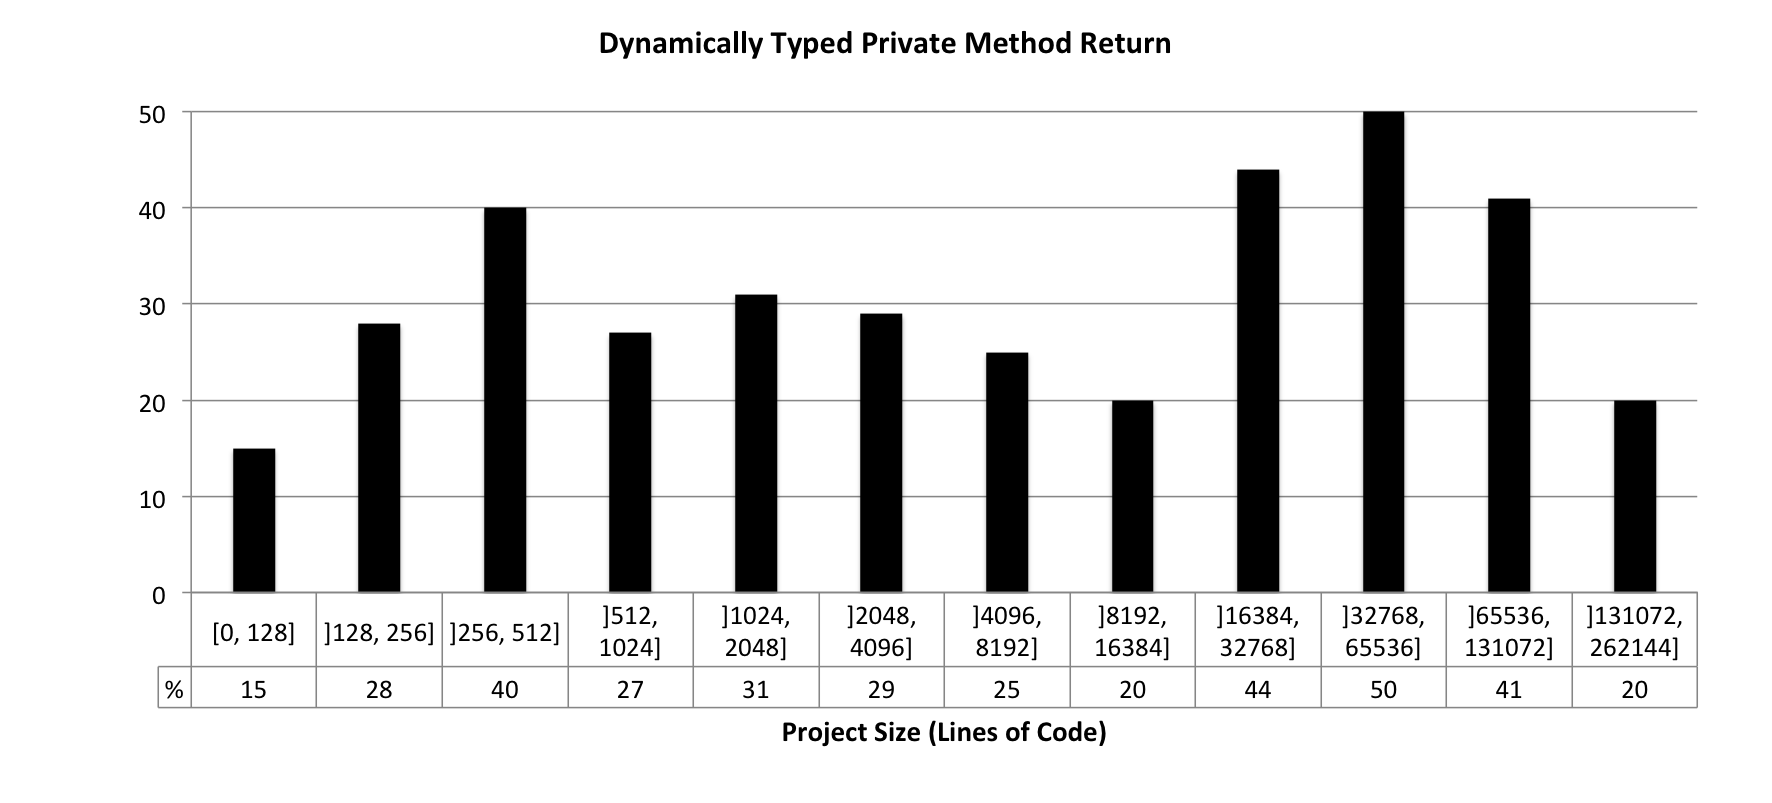
\includegraphics[width=1\textwidth]{images/size_priMethodReturn} 
\caption{Untyped private declarations}
\label{fig:size_priMethodReturn} 
\end{figure*}

\begin{figure*}[ht]
\centering 
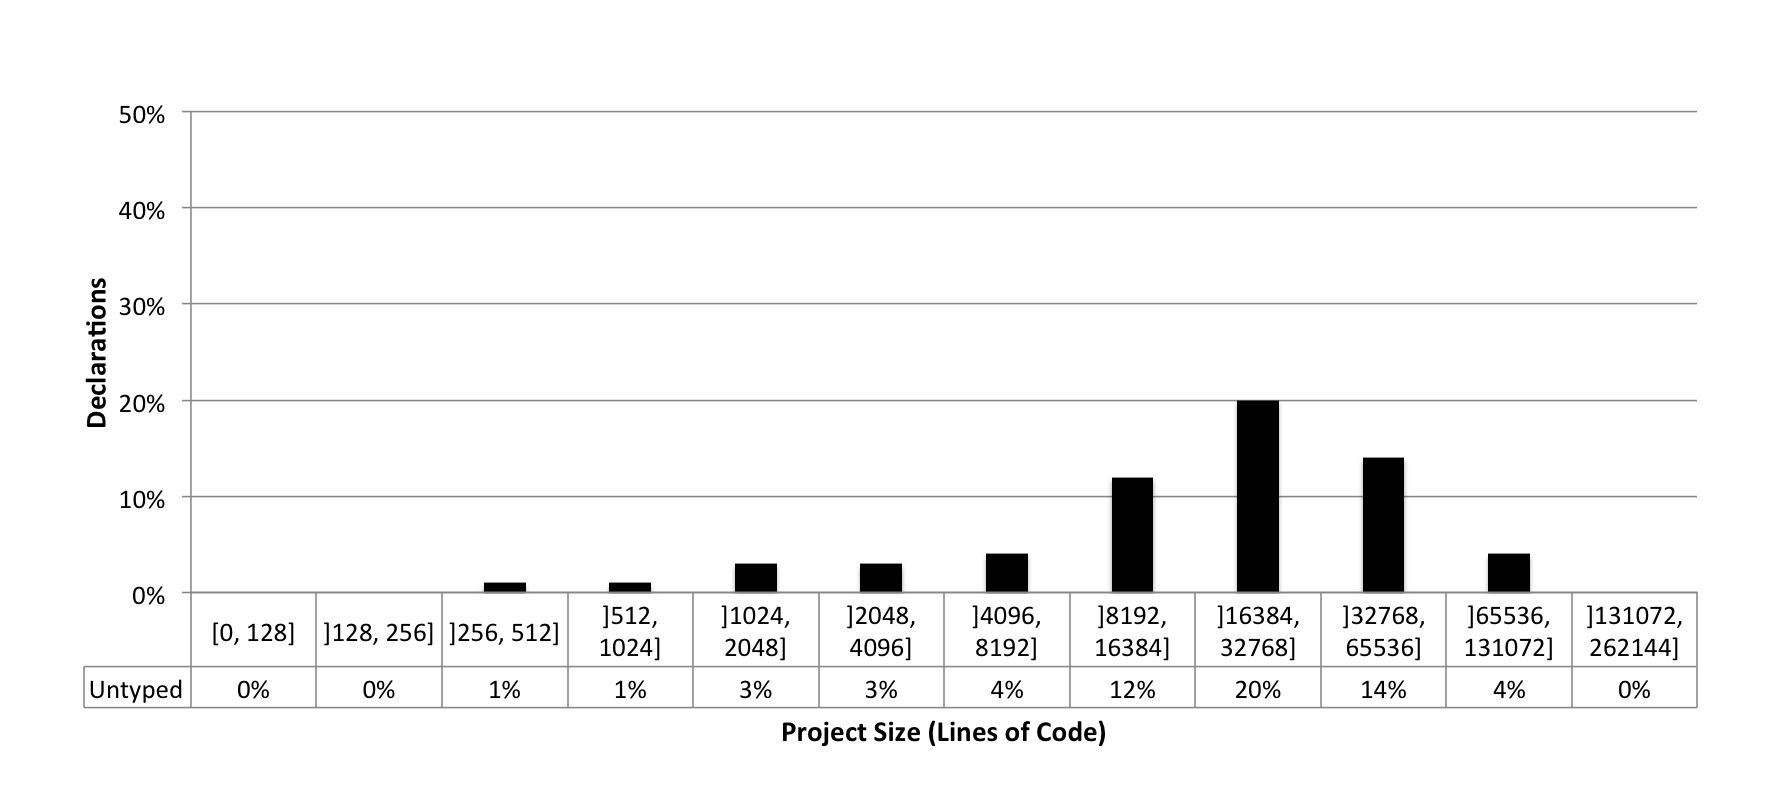
\includegraphics[width=1\textwidth]{images/size_proMethodReturn} 
\caption{Untyped private declarations}
\label{fig:size_proMethodReturn} 
\end{figure*}

Conversely, the use of untyped declarations in local variables increases with the project size. 
This is shown in Figure \ref{fig:size_localVariable}. 
The average frequency of untyped local variable declarations in projects with less than $512$ lines of code is less than $40\%$. 
On the other side, in projects with over $65536$ lines of code, the average frequency for this type of declaration exceeds $70\%$.

\begin{figure*}[ht]
\centering 
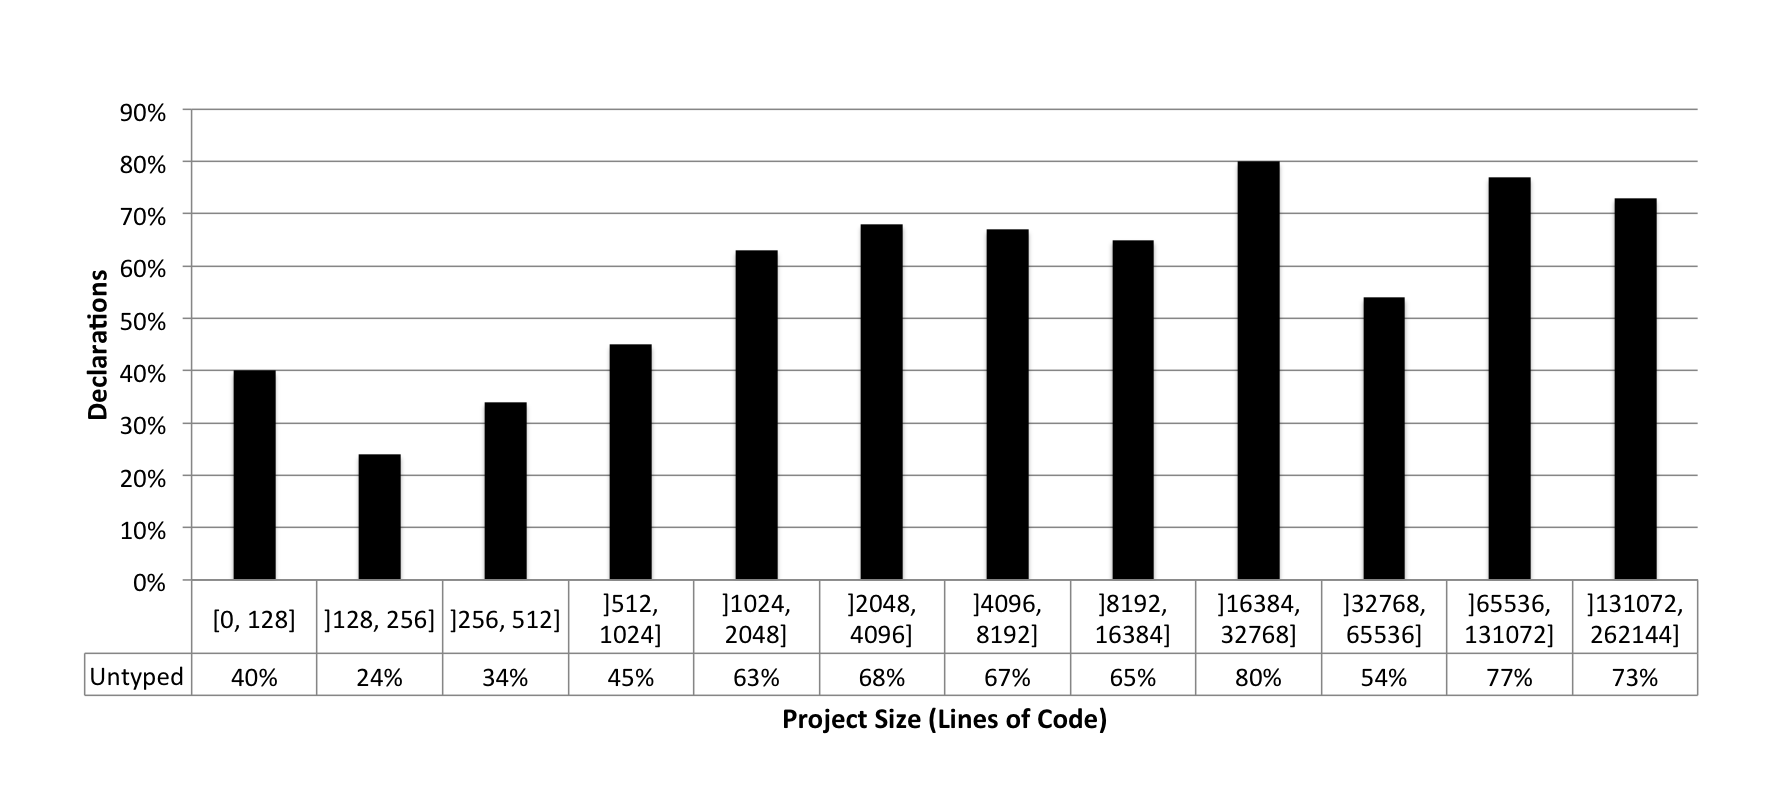
\includegraphics[width=1\textwidth]{images/size_localVariable} 
\caption{Untyped local variables}
\label{fig:size_localVariable} 
\end{figure*}





















%
% DISCUSSION
%
\section{Discussion\label{discussion}}
In this section, we discuss the questions proposed in Section \ref{questions} based on the results above.
We were able to find evidence to support an affirmative answer for all 3 questions.
Section \ref{discussion-q1} shows that documentation is the main reason why Groovy developers use types, specially on the definition of their modules.
An analysis of local variables, private statements and test classes in Section \ref{discussion-q2} supports the suspect that untyped declarations are used more frequently when readability or stability aren't a concern. 
Last, Section \ref{discussion-q3} shows how programmers with experience on statically typed languages use types more frequently than other programmers.

% Q1
\subsection{Types as implicit documentation\label{discussion-q1}}
Well documented code plays an important role in making code more readable, hence improving the code overall maintainability \cite{Iso2004}.
By analyzing the results presented in Section \ref{sec:results}, we were able to find evidence that this is an important factor considered by Groovy programmers.

Documentation is the main reason why Groovy programmers type their code.
It is well known that the main advantages of using statically typed languages are implicit code documentation, static type verification and execution performance.
Groovy however is not a statically typed language, but a dynamically typed language with optional typing (we are not considering the $@TypeChecked$ annotation in this study).
This means that Groovy compiler can't verify types statically and that types still have to be checked during execution, which degrades runtime performance.
Hence from the usual advantadges of using a statically typed language, only code documentation holds true for Groovy.
Considering the result shown on previous section, which shows that 60\% of all declarations are typed, this means that code documentation is an important matter for Groovy developers.

It is possible to observe an even higher usage of typing in the definition of modules.
As mentioned in the literature \cite{Meyer88, Meijer04, Wadler04, Plosch97, Flanagan2006, Furr09}, types greatly aid in the definition of the contract of a module.
They restrict the pre and post conditions of methods and define the nature of the properties of that module.
Clients of an well typed module learn how to use it faster and make less mistakes since the contract of that module is clear to them.

Statements that define the interface of a module, i.e, fields, returns and parameters of methods and parameters of constructors, are more typed than the average.
Consider Figure \ref{fig:tipo_declaracao}.
While most of these elements are typed, only 30\%  of the local variables, which do not contribute to the definition of a module, are typed. On the other side, parameters of constructors, which are some of the most important elements of a contract definition, are almost always typed

Section \ref{sub:visibility-results} further refines the results presented above.
Figures \ref{fig:method_return_visibility}, \ref{fig:method_parameter_visibility}, \ref{fig:constructor_parameter_visibility} and \ref{fig:field_visibility} show how programmers type their declarations by visibility.
These results contribute to the understanding that types are indeed considered more often on the definition of modules.
First, notice that private statements are always less typed than their public and protected counterparts.
Private statements are similar to local variables since they do not contribute to the interface of a module and are only accessible to the module where they were defined.
In this case there is a smaller need for documentation and programmers do not feel as compelled to use types.

Public and protected elements define the interface of a method and thus are widely typed.
In the case of parameters and returns of methods, the usage of types in statements with protected visibility  surpasses that of statements with public visibility.
In Groovy, protected declarations restrict access to internal elements of a class to its subclasses or other classes in the same package.
It can be argued that the relationship between these classes is tightly coupled \cite{Eder94}.
Apparently programmers understand that this type of contract is more delicate than others and that it should be well document.

The usage of types in public declarations is heavily influenced by the project size.
Figure \ref{fig:size_pubMethodReturn} shows this clearly.
In projects with more than 65KLoC, these untyped declarations are seen with less than half the frequency observed in the smallest projects.
However, no particular pattern can be observed for private or protected declarations, represented by Figures \ref{fig:size_priMethodReturn} and \ref{fig:size_proMethodReturn}.

Intuitively, the larger the project, the greater the difficulty of integration and the need for maintenance.
This is more critical in public statements.
Unlike private or protected statements, the number of modules to which a public statement is visible grows with the project size.
This suggests that as projects grow, programmers realize that the documentation of public elements is more important and consider typing these declarations more often.

The project size has an opposite effect on the declarations of local variables.
While public declarations get typed more often, the frequency of types in local variable declarations decreases.
It is hard to tell the reason for this behavior.
A possible explanation is that, as project grows, developers get more used to flexibility and objectivity of dynamic typing.
They stop typing their declarations unless they understand they are really necessary.

% Q2
\subsection{Less typing when readability and stability aren't a concern\label{discussion-q2}}
When readability or stability are not a concern, the advantages of typing become less apparent and  programmers prefer the flexibility and objectivity of untyped declarations.
This is what we found when we analyzed how typing is used in local variables, private statements and test classes.
These are scenarios we consider readability and stability to be less relevant.

Most local variables are untyped.
Figure \ref{fig:tipo_declaracao} shows that less than 30\% of these variables are declared with a type, a value significantly smaller than the overall result for all declaration types, 60\%.
It can be assumed that typing local variables does not aid in the readability of the code as much as in other types of declarations.
The value of a local variable is defined very close to its declaration, usually in the same statement.
This makes it easier for a reader to understand the nature of a given variable and even infer its type.
Programmers can be more objective in this scenario and eliminate the repetitive work of typing their variables.

Local variables have a smaller scope and life cycle.
They are only visible inside the block where they were instantiated and are destroyed once the execution of that block is over.
Stability in this scenarios is not as critical making the flexibility of untyped declarations more apparent.
For example, one can easily change the type of a local variable without having to worry about its use anywhere else.

A similar conclusion can be derived for private statements.
As shown in Figures \ref{fig:method_return_visibility}, \ref{fig:method_parameter_visibility}, \ref{fig:constructor_parameter_visibility} and \ref{fig:field_visibility}, untyped declarations are much more common in in these statements that in their public or private counterparts.
Private statements are usually more stable than others.
Since they are only visible inside the class they were defined in, they can often be changed without having any unexpected effects outside that class.
Also, since those statements are only referenced inside the class where they were defined, a reader can easily find those references and use them as a means to understand the code.

Another scenario with smaller need for readability and stability are test classes.
These classes usually have simple relationships with the rest of the project, not having any clients and depending only on the classes under test.
Test code is frequently considered a peripheral artifact of a software project and programmers usually do not worry about keeping the quality of such code \cite{Meszaros07}.

Test classes are also typed less often than the usual.
Figure \ref{fig:tests} shows that declarations made inside the main classes of a project are typed in 68\% of the cases.
On the other side, only 56\% of the test classes are typed.

A counter example to this analysis is the usage of types in scripts.
It can also be said that readability and stability are not big concerns in scripts.
These are pieces of code usually written to solve punctual problems.
They do not establish complex relationships with other modules and aren't reused very often.
Nevertheless, as shown in Table \ref{fig:scripts}, there is no significant difference between the overall usage of types in scripts and classes.


% Q3
\subsection{Previous experience of programmers\label{discussion-q3}}
Results indicate that the answer for Q3 is affirmative.
The choice for using types on a language with optional typing, such a Groovy, is in fact influenced by the experience  with other languages.
Those developers who have only static languages on their GitHub portfolio leave their statements untyped less often than other developers.
Figure \ref{fig:untyped_background} shows that these developers have only 28.7\% of their statements untyped compared to 40\% of those developers with dynamic languages on their portfolio. 

It is clear that the portfolio of a GitHub developer might not represent well his real experience with other programming languages.
This developer might have projects hosted somewhere else or have projects in his portfolio that he has barely participated at.
However, due to the scale of this study, it is difficult to collect more detailed metrics for every user.











%
% THREATS TO VALIDITY
%
\section{Threats to Validity\label{threats}}
In this section, we discuss potential threats to validity. As usual, we have arranged possible threats in two categories, internal and external validity \cite{Wohlin2012}. The main threats to the internal validity of this work involve the fact that, in such a large scale case study, we can't analyze data into much detail. In Section \ref{sub:background} we consider that the GitHub portfolio of a programmer represents well his experience with other languages and type systems.
However, these programmers might have projects hosted somewhere else or projects in his portfolio that he hasn't worked on.
In Section \ref{sub:size-results}, we consider that the project size is a metric capable of representing the complexity of a project well.
This is not always true \cite{Fenton1998}, but that was the most effective metric we could use without requiring projects to be compiled, which would drastically reduce our dataset.

There are other variables that can have influenced the programmers besides the ones considered in this study.
Some frameworks require programmers to use typed or untyped declarations in some cases.
For example, one of the ways a programmer can create a mock on Spock, a popular Groovy testing framework, requires programmers to type the mock declaration.
Also, tool integration might encourage programmers to use types for functionalities such as code completion.
In addition to that, the previous experience of programmers, which we have shown to have influence over programmers, might interfere with analyzis of other influencing factors.

In order to overcome the threats shown above, as a future work, we are planning a controlled study.
This will provide us with more detailed information, which we can use to complement the results of this case study.

As threts to external validity, 
% .. 

The results presented in this study can not be generalized for every scenario.
Depending on the context, each developer might find different reasons to type or not their declarations.
Also, since we only analyzed public projects, we can not say that our dataset can represent projects developed inside an organization, which are mostly private projects.







%
% RELATED WORK
%
\section{Related Work\label{sec:Trabalhos-Relacionados}}
This work is based on a series of studies that compare different typing strategies.
Although we are not aware of any studies that analyze this question using a large scale case study as ours, we are aware of multiple controlled experiments with significant results.

In \cite{experiment_with_purity}, the author compares the performance of two groups of students asked to develop two small systems. 
Both groups used a language developed by the author, Purity. 
The only difference in the language used by the two groups was the typing system.
One group used a statically typed version of Purity while the other used a dynamically typed version of the same language.
Results showed that the group using the dynamic version was significantly more productive than the other. 
Similarly to this work, the author was able to compare two typing strategies directly while isolating any external factors. 
However, it can be argued that these results may not represent well real life situations of the software industry. 
This was a short duration study where students were used as examples of developers with no interaction with other programmers. 
In our study, we try to get more relevant results when analyzing source code developed by programmers during their normal activities.

In a follow up study \cite{hanenberg_icpc}, the authors got to opposite conclusions. 
They compared the performance of two groups of developers in maintenance tasks. 
The first group used Java, a statically typed language, and the other used Groovy, but restricting developer to use only untyped declarations in order to simulate a dynamically typed version of Java.
In this case, the group using the statically typed language, Java, was much more productive.
This contradiction with a previous work reinforces the argument that the results of controlled studies aren't reliable enough for this type of study.

In experiments conducted in \cite{ruby_vs_druby}, the authors compare the performance of two groups working on small development tasks.
One group used Ruby, a dynamically typed language, while the other used DRuby, a statically typed version of Ruby. 
Results showed that the DRuby compiler rarely managed to capture any errors that weren't already evident for programmers.
Most subjects involved in the study had previous experience with Ruby, which suggests that programmers get used to the lack of typing in their declarations.
We tried to investigate this phenomenon, by analyzing how programmers use types depending on their experience with other languages.











%
% CONCLUSION AND FUTURE WORK
%
\section{Conclusions and Future Work\label{conclusion}}
In this study, we investigated, from a practical point of view, what are the most influential factors on the choice of a programmer for using or not types.
Understanding these factors can help programmers choosing the most appropriate programming language for a given context.
It's also a valuable information for programming language designers who can base their design on real user data.
To answer this question, we conducted a large scale case study with more that 7 thousand software projects written in Groovy, a dynamically typed language with optional type annotations. 

We found evidence that programmers use types as a means to implicitly document their code.
This tends to grow in the presence of some factors, such as the statement visibility, the complexity of the contract defined by such statement and the size of the project where it is defined. 
Conversely, when readability or stability aren't a concern, the simplicity and flexibility of untyped declarations seems to be preferred, as seen on local variables, private statements and test classes.
Another important factor is the previous experience of programmers with a given type system.

In future works we wish to analyze the influence of static and dynamic type systems over the robustness of software systems.
In particular , we want to understand whether the use of dynamic typing, which limits the compiler's ability to find type problems, has any correlation with the occurrence of defects in the system and if the use of automated testing is able to reduce this correlation.

\acks
This work was partially supported by FAPEMIG, grants APQ-02376-11 e APQ-02532-12, and CNPq grant 485235/2011-0. 


%
% BIBLIOGRAPHY
%
\bibliographystyle{abbrvnat}
\renewcommand{\bibfont}{\normalsize}
\begin{thebibliography}{}
\softraggedright

\bibitem[Tiobe Website(2013)]{tiobe}
Tiobe programming community index. http://www.tiobe.com/index.php/ content/paperinfo/tpci/index.html. Accessed in 23/09/2013.

\bibitem[Groovy(2013)]{groovy}
Groovy Programming Language. http://groovy.codehaus.org/. Accessed in 10/10/2013.

\bibitem[Bruce, K. (2002)]{bruce2002foundations}
Bruce, K. (2002). Foundations of object-oriented languages: types and semantics. MIT press.

\bibitem[Bruch, M., Monperrus, M., and Mezini, M. (2009)]{bruch2009learning}
Bruch, M., Monperrus, M., and Mezini, M. (2009). Learning from examples to improve code completion systems. In Proceedings of the the 7th joint meeting of the European software engineering conference and the ACM SIGSOFT symposium on The foundati- ons of software engineering, pages 213–222. ACM.

\bibitem[Cardelli, L. (1996]{type_systems}
Cardelli, L. (1996). Type systems. ACM Comput. Surv., 28(1):263–264.

\bibitem[Chang, M., Mathiske, B., Smith, E., Chaudhuri, A., Gal, A., Bebenita, M., Wimmer, C.]{jit}
Chang, M., Mathiske, B., Smith, E., Chaudhuri, A., Gal, A., Bebenita, M., Wimmer, C., and Franz, M. (2011). The impact of optional type information on jit compilation of dynamically typed languages. SIGPLAN Not., 47(2):13–24.

\bibitem[Daly, M. T., Sazawal, V., and Foster, J. S. (2009)]{ruby_vs_druby}
Daly, M. T., Sazawal, V., and Foster, J. S. (2009). Work In Progress: an Empirical Study of Static Typing in Ruby. In Workshop on Evaluation and Usability of Programming Languages and Tools (PLATEAU), Orlando, Florida.

\bibitem[Hanenberg, S. (2010)]{experiment_with_purity}
Hanenberg, S. (2010). An experiment about static and dynamic type systems: doubts about the positive impact of static type systems on development time. SIGPLAN Not., 45(10):22–35.

\bibitem[Kleinschmager, S., Hanenberg, S., Robbes, R., and Stefik, A. (2012)]{hanenberg_icpc}
Kleinschmager, S., Hanenberg, S., Robbes, R., and Stefik, A. (2012). Do static type systems improve the maintainability of software systems? An empirical study. 2012 20th IEEE International Conference on Program Comprehension (ICPC), pages 153– 162.

\bibitem[Lamport, L. and Paulson, L. C. (1999)]{should_your_specification_language_be_typed}
Lamport, L. and Paulson, L. C. (1999). Should your specification language be typed. ACM Trans. Program. Lang. Syst., 21(3):502–526.

\bibitem[Mayer,C.,Hanenberg,S.,Robbes,R.,Tanter,E ́.,andStefik,A.(2012)]{mayer2012static}
Mayer,C.,Hanenberg,S.,Robbes,R.,Tanter,E ́.,andStefik,A.(2012). Static type systems (sometimes) have a positive impact on the usability of undocumented software: An empirical evaluation. self, 18:5.

\bibitem[Pierce, B. (2002)]{types_and_programming_languages}
Pierce, B. (2002). Types and programming languages. MIT press.

\bibitem[Tratt, L. (2009)]{dynamically_typed_languages}
Tratt, L. (2009). Chapter 5 dynamically typed languages. volume 77 of Advances in Computers, pages 149 – 184. Elsevier.

\bibitem[Siek, Jeremy, and Walid Taha(2007)]{gradual_typing}
Siek, Jeremy, and Walid Taha. "Gradual typing for objects." ECOOP 2007–Object-Oriented Programming. Springer Berlin Heidelberg, 2007. 2-27.

\bibitem[Gray(2008)]{gray08}
Gray, K. E. Safe cross-language inheritance. In European Conference on Object-Oriented Programming (2008), pp. 52–75.

\bibitem[Gray(2011)]{gray11}
Gray, K. E. Interoperability in a scripted world: Putting inheritance \& prototypes together. In Foundations of Object-Oriented Languages (2011).

\bibitem[Gray(2005)]{gray05}
Gray, K. E., Findler, R. B.,Andflatt, M. Fine-grained interoperability through contracts and mirrors. InObject-Oriented Programming, Systems, Languages, and Applications(2005), pp. 231–245.

\bibitem[Siek(2007)]{siek07}
Siek, J.,Andtaha, W. Gradual typing for objects. In European Conference on Object-Oriented Programming(2007),pp. 2–27.

\bibitem[Takikawa(2012)]{takikawa12}
Takikawa, Asumu, et al. "Gradual typing for first-class classes." ACM SIGPLAN Notices. Vol. 47. No. 10. ACM, 2012.
\bibitem[Fowler(2010)]{fowler10}
Fowler, Martin. Domain-specific languages. Pearson Education, 2010.

% Types help on the definition of a contract
\bibitem[Meijer(2004)]{Meijer04}
Meijer, Erik, and Peter Drayton. "Static typing where possible, dynamic typing when needed: The end of the cold war between programming languages." OOPSLA, 2004.

\bibitem[Wadler(2004)]{Wadler04}
Wadler, Philip, and Robert Bruce Findler. "Well-typed programs can’t be blamed." Programming Languages and Systems. Springer Berlin Heidelberg, 2009. 1-16.

% Unfortunately, dynamically typed programming languages usually do not support the concept of DEC. Therefore we integrated DEC into the programming language Python by using a metaprogramming approach
\bibitem[Plosch(1997)]{Plosch97}
Plosch, Reinhold. "Design by contract for Python." Software Engineering Conference, 1997. Asia Pacific and International Computer Science Conference 1997. APSEC'97 and ICSC'97. Proceedings. IEEE, 1997.

%Traditional static type systems are very effective for verifying basic interface specifications
\bibitem[Flanagan(2006)]{Flanagan2006}
Flanagan, Cormac. "Hybrid type checking." ACM Sigplan Notices. Vol. 41. No. 1. ACM, 2006.

\bibitem[Meyer(1988)]{Meyer88}
Meyer, Bertrand. Object-oriented software construction. Vol. 2. New York: Prentice hall, 1988.

\bibitem[Furr(2009)]{Furr09}
Furr, Michael, et al. "Static type inference for Ruby." Proceedings of the 2009 ACM symposium on Applied Computing. ACM, 2009.

\bibitem[Meszaros(2007)]{Meszaros07}
Meszaros, Gerard. xUnit test patterns: Refactoring test code. Pearson Education, 2007.

% Coupling is high for inheritance
% interaction coupling, component coupling and inheritance coupling
\bibitem[Eder(1994)]{Eder94}
Eder, Johann, Gerti Kappel, and Michael Schrefl. "Coupling and cohesion in object-oriented systems." Technical Reprot, University of Klagenfurt, Austria (1994).

\bibitem[ISO25000(2004)]{Iso2004}
ISO, ISO, and IEC FCD. "25000, Software Engineering-Software Product Quality Requirements and Evaluation (SQuaRE)-Guide to SQuaRE." Geneva, International Organization for Standardization (2004).

\bibitem[Fenton(1998)]{Fenton1998}
Fenton, Norman E., and Shari Lawrence Pfleeger. Software metrics: a rigorous and practical approach. PWS Publishing Co., 1998.

\bibitem[Wohlin(2012)]{Wohlin2012}
Wohlin, Claes, et al. Experimentation in software engineering. Springer Publishing Company, Incorporated, 2012.

\end{thebibliography}


\end{document}

%                       Revision History
%                       -------- -------
%  Date         Person  Ver.    Change
%  ----         ------  ----    ------

%  2013.06.29   TU      0.1--4  comments on permission/copyright notices

